\documentclass[border=5pt]{standalone}
\usepackage{pgfplots}
\pgfplotsset{compat=1.18} % Рекомендуется использовать актуальную версию

\begin{document}
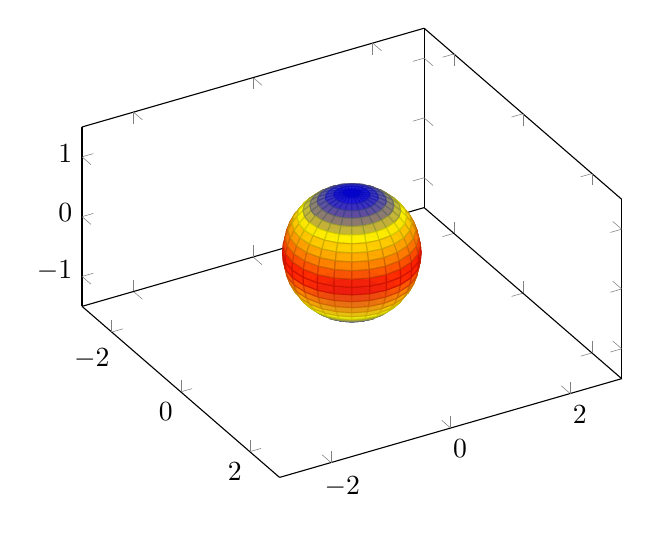
\begin{tikzpicture}
  \begin{axis}[
    view={60}{30}, % Угол обзора (азимут, угол возвышения)
    axis equal,    %<--- Это ключевая настройка!
    xmin=-1.5, xmax=1.5,
    ymin=-1.5, ymax=1.5,
    zmin=-1.5, zmax=1.5,
    %xlabel={$x$}, ylabel={$y$}, zlabel={$z$},
    colormap={periodic}{
      color=(blue)
      color=(yellow)
      color=(orange)
      color=(red)
      color=(orange)
      color=(yellow)
      color=(blue)
    },
    samples=25,
  ]
  
  \addplot3[
    surf,
    domain=0:pi,        % Верхняя полусфера
    y domain=0:2*pi,
    z buffer=sort,
    opacity=0.9
  ] (
    {sin(deg(x)) * cos(deg(y))},
    {sin(deg(x)) * sin(deg(y))},
    {cos(deg(x))}
  );

  \addplot3[
    surf,
    domain=pi:2*pi,     % Нижняя полусфера
    y domain=0:2*pi,
    z buffer=sort,
    opacity=0.9
  ] (
    {sin(deg(x)) * cos(deg(y))},
    {sin(deg(x)) * sin(deg(y))},
    {cos(deg(x))}
  );
  \end{axis}
\end{tikzpicture}
\end{document}